В командной части заключительного этапа участники должны
разработать децентрализованное приложение на базе платформы Ethereum,
для взаимодействия автономных электромобилей и автоматических станций
сервисного
обслуживания, предоставляющих услуги по замене разряженных  
тяговых аккумуляторных батарей. Приложение включает в себя логику
проверки батарей на контрафакт, а также экономическую систему мотивации
участия и защиты от мошенничества.

Командная часть заключительного этапа имеет продолжительность
3.5 дня (всего 24 астрономических часа), которые включают работу по
настройку среды разработки на базе узла сети Ethereum, разработку
частей приложения на языке Python и Solidity, создание интеграционных
тестов, а также приемка решения в системе автоматической проверки.

\section{Легенда}
Недалёкоое будущее, в автоматических логистических центрах практически нет людей, всю работу
выполняют роботы-погрузчики, которыми управляет интеллектуальное ПО по распределению задач.

Несмотря на отсутствие человеческого фактора, не следует думать, что в таких
центрах никогда не будет проблем. Форс-мажор может произойти в любой момент и система
из роботов и ПО должна уметь справляться с такими ситуациями.

Поэтому для финальной задачи профиля <<Интеллектуальные робототехнические системы>>
предлагается рассмотреть следующий эпизод: в логистическом центре произошла перезагрузка
всех систем, что привело к сбросу информации о местоположениях работающих в данный момент роботов-погрузчиков.

В начале выполнения задания считается, что робототехнические устройства активируются
в каких-то секторах (каждый в своём) логистического центра.
При этом 2 из них имеют информацию о своём местоположении,
а у 3-го была повреждена память и по этому эта информация была потеряна.
Структура логистического центра известна заранее всем устройствам.
Роботы-погрузчики должны переместиться в сектор своей приписки.
Координаты секторов сервисного обслуживания известны заранее.
Информацию о местоположении необходимого сектора приписки можно узнать в
секторе сервисного обслуживания. В нём располагается ARTag маркер, в котором закодирован номер робота и
координаты сектора его приписки. При перемещении роботы не должны сталкиваться, а
также повреждать логистический центр.


Задача участников Олимпиады --- разработать программу управления несколькими робототехническими
устройствами для выполнения задания описанного выше.

\putImgForRef{16cm}{sources/NTI_IRS_2019_field.jpg}
{Полигон для запуска робототехнических устройств на финале Олимпиады НТИ}{fig:NTI-IRS-2019-field}


\section{Набор заданий}

Решение командной задачи разбито на 5 этапов. Первые четыре
этапа итеративно подводят участников к решению полной финальной
задачи, осуществляемому во время последнего пятого этапа. На
каждом этапе в проверку решения заданий данного этапа входят:
\begin{itemize}
    \item способность проверить гипотезу о работоспособности алгоритма
    через демонстрацию решения в симуляторе;
    \item полнота решения задания конкретного этапа;
    \item воспроизводимость результатов --- робототехническое
    устройство участников должно было неоднократно выполнить требуемые
    действия.
\end{itemize}

\subimport{final/command_tour/telecom/}{intro.tex}

\chapter{Задачи}

\subimport{final/command_tour/telecom/task_01/}{statement.tex}
\subimport{final/command_tour/telecom/task_01/}{solution.tex}

\subimport{final/command_tour/telecom/task_02/}{statement.tex}
\subimport{final/command_tour/telecom/task_02/}{solution.tex}

\subimport{final/command_tour/telecom/task_03/}{statement.tex}
\subimport{final/command_tour/telecom/task_03/}{solution.tex}

\subimport{final/command_tour/telecom/task_04/}{statement.tex}

\subimport{final/command_tour/telecom/task_05/}{statement.tex}

\subimport{final/command_tour/telecom/}{criteria.tex}

\section{Описание модели логистического центра}
Полигон - квадратное поле $3200\times3200$ мм., разделенное на квадратные сектора $400 \times 400$ мм.
Некоторые сектора отделены друг от друга перегородкой высотой $100$ мм.
Некоторые сектора недоступны для посещения робототехническим устройством и представляют из себя 
модель стеллажа высотой $210$ мм.
На каждой полке стеллажа располагается черный контейнер с грузом ~(рис.~\ref{fig:container}) размером
$200 \times 300 \times 100$ мм (груз - 2-3 коробки~(рис.~\ref{fig:box}) размером $180 \times 80 \times 85$ мм).


\begin{figure}[h]
\begin{center}
\begin{minipage}[h]{0.5\linewidth}

\includegraphics[width=1\linewidth]{sources/container}
\caption{Внешний вид контейнера}
\label{fig:container} 
\end{minipage}
\hfill 
\begin{minipage}[h]{0.4\linewidth}
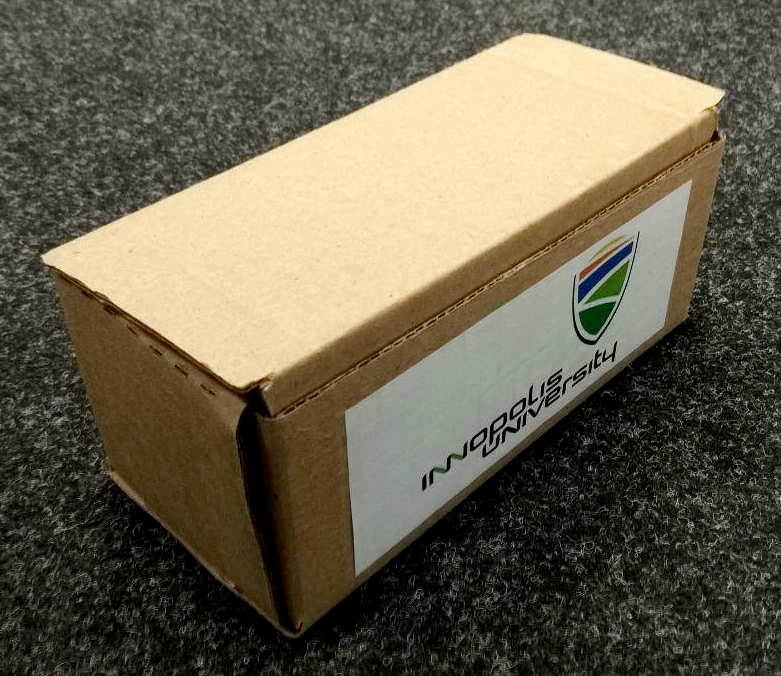
\includegraphics[width=1\linewidth]{sources/box}
\caption{Внешний вид коробки}
\label{fig:box}
\end{minipage}
\end{center}
\end{figure}

Полигон окружен бортом высотой $100$ мм.
Конфигурация полигона определяется в первый день финального этапа и объявляется участникам.
Данная конфигурация будет использоваться во все дни финального этапа.

На нижней полке стеллажа, прилегающего одной из четырех сторон к сектору сервисного обслуживания,
на высоте от 100-150 мм от уровня поверхности поля закреплен ARTag маркер (\url{https://goo.gl/WaTFMB}),
определяющий номер робота и координаты сектора приписки (сектор финиша для конкретного робота).
Размер маркера - $30\times30$ мм.
Маркер обращен лицевой стороной внутрь сектора сервисного обслуживания, координаты которого известны заранее.
Конкретная высота расположения маркеров определяется в первый день финала и остается
постоянной во все дни финального этапа. При этом допустимая погрешность установки
маркеров $\pm 5$ мм. Пример расположения маркера на стелаже представлен на рисунке \ref{fig:cellInARTag}

\putImgForRef{8cm}{sources/cell-with-ARTag.jpg}
{Стеллаж с установленным ARTag маркером}{fig:cellInARTag}

Маркер состоит из $6\times6$ элементов одинакового размера.
Элементы маркера, расположенные по его границе --- всегда черные. Четыре элемента,
находящиеся в углах внутреннего $4\times 4$ квадрата определяют ориентацию маркера таким
образом, что только один из них --- белый.
Оставшиеся $12$ элементов маркера кодируют число по следующему правилу: если элемент черный, то в он обозначает $1$, если белый,
то $0$ при этом самый первый элемент --- старший бит закодированного числа.
Нумерация элементов относительно ориентационных элементов обозначена на рисунке \ref{fig:marker-bits}.

\putImgForRef{5cm}{sources/artag-about}
{Нумерация элементов маркера относительно ориентационных элементов}{fig:marker-bits}


\putImgForRef{5cm}{sources/artag-ex1}
{Маркер с закодированным значением - $010011100101_2$}{fig:marker-ex1}


Закодированное на маркере двоичное двенадцатибитное число закодировано с использованием кода Хэмминга (https://habr.com/ru/post/140611/), в котором 8 информационных битов
и 4 контрольных бита:
\begin{enumerate}
    \item[1] Первый контрольный бит;
    \item[2] Второй контрольный бит;
    \item[3] Старший бит номера робота $N$($1 \leq N \leq 3$);
    \item[4] Третий контрольный бит;
    \item[5] Младший бит номера робота $N$($1 \leq N \leq 3$);
    \item[6] Первый (старший) бит координаты $X$ робота $N$ ($0 \leq X_N \leq 7$);
    \item[7] Второй бит координаты $X$ робота $N$ ($0 \leq X_N \leq 7$);
    \item[8] Четвёртый (последний) контрольный бит;
    \item[9] Третий (младший) бит координаты $X$ робота $N$ ($0 \leq X_N \leq 7$);
    \item[10] Первый (старший) бит координаты $Y$ робота $N$ ($0 \leq Y_N \leq 7$);
    \item[11] Второй бит координаты $Y$ робота $N$ ($0 \leq Y_N \leq 7$);
    \item[12] Третий (младший) бит координаты $Y$ робота $N$ ($0 \leq Y_N \leq 7$);
\end{enumerate}


Маркер на рисунке \ref{fig:marker-ex1} кодирует число $010011100101_2$ --- $N = 1$, $X = 6$, $Y = 5$.
Таким образом, сектор приписки для робота $1$ находится в позиции с координатами $(6, 5)$ --- см. рисунок \ref{fig:sector-example}.


\putImgForRef{9cm}{sources/sector-example}
{Расположение сектора финиша для маркера из рисунка \ref{fig:marker-ex1}}{fig:sector-example}

Гарантируется, что сектора сервисного обслуживания будут располагаться в таких
местах полигона, где к сторонам сектора прилегает как минимум один стеллаж.

Сектора активаций роботов (стартов), сектора сервисного обслуживания и сектора приписки никак
не обозначаются на поле и определяются непосредственно перед каждым заездом робота.



\section{Описание конструктора}
\putImgForRef{8cm}{final/command_tour/irs/sources/TRIK_IRS_mobile_vehicle.jpg}
{Мобильная платформа TRIK в сборе}{fig:TRIK-IRS-mobile-vehicle}

В первый день финального тура каждой команде выдаются три комплекта:
\begin{itemize}
    \item Мобильная наземная платформа на базе конструктора TRIK в сборе
    (блок управления TRIK, аккумулятор, два мотора с энкодерами на датчиках
    Холла, колеса), но без установленных датчиков.
    Мобильная платформа построена по принципу дифференциального управления.
    Физические размеры платформы позволяют совершать все маневры внутри одного сектора
    модели логистического центра без касания со стенками стеллажей или бортов.
    \item Комплект дополнительных деталей из конструктора TRIK и набор датчиков:
    2 инфракрасных датчика дальности, 2 ультразвуковых датчика расстояния и 1 VGA-камера;
    \item комплект дополнительных деталей из конструктора TRIK;
    \item Ноутбуки с установленной TRIK Studio, каждой команде по одному ноутбуку.
    При этом участники могут пользоваться своими ноутбуками.

\end{itemize}

\section{Условия проведения}
\begin{itemize}
    \item В первые день соревнований все члены команд получают ноутбук со следующим набором
    установленного программного обеспечения:
    \begin{itemize}
        \item набор Python инструментария Anaconda c установленными библиотеками \texttt{web3} (\texttt{v5.0.0a3}), \texttt{cognitive\_face}, \texttt{opencv-python};
        \item среды разработки PyCharm и WingIDE;
        \item компилятор языка Solidity \texttt{solc} (\texttt{v0.5.4});
        \item клиент системы ведения версий \texttt{git};
        \item Интернет-браузер Chrome.
    \end{itemize}
    Каждый ноутбук имеет возможность выхода в сеть Интернет. Команды могут использовать
    собственные ноутбуки.

    \item Команды могут устанавливать дополнительное программное обеспечение, но после
    согласования с членами жюри.

    \item Участники во время командного этапа финального тура могут использовать интернет
    и заранее подготовленные библиотеки для решения задачи.

    \item Участники должны использовать язык программирования Python для написания
    программ, использующих командную строку. Для написания Ethereum контрактов
    участники могут использовать любой язык программирования.

    \item Для работы с сервисом \textit{Microsoft Face API} участникам предоставляется
    один ключ подписки на команду, а также базовый URL для доступа к REST API. При
    доступе к сервису с помощью данного ключа действует ограничение на 10 запросов в
    секунду. Участники одной команды должны сами заботиться о том, чтобы держать ключ
    в тайне от других команд. Ключ не должен передаваться третьим лицам. Если ресурс
    ключа подписки (примерно 60000 запросов) полностью используется командой, то
    организаторы вправе не предоставлять команде другой ключ.

    \item Участники не могут использовать помощь тренера, сопровождающего лица или
    привлекать третьих лиц для решения задачи.

    \item Финальная задача формулируется участникам в первый день финального тура,
    но участники выполняют решение  задачи поэтапно. Критерии прохождения каждого
    этапа формулируются для каждого дня финального тура. За подзадачи, решенные в
    конкретном этапе начисляются, баллы. Баллы за подзадачи можно получить только
    в день, закрепленный за конкретным этапом.

    \item В начале первого дня состязаний участники каждой команды получают доступ 
    к репозиторию на серверах GitLab.com. Каждая команда имеет свой собственный 
    репозиторий. Члены других команд не имеют доступ к чужим репозиториям.

    \item В течение дня не ведется учет количества изменений, которые команды
    регистрируют в Git-репозитории.

    \item В конце каждого дня финального этапа жюри проверяет решение участников
    на соответствие приемочным тестам для каждой подзадачи, входящей в набор
    для соответствующей итерации.

    \item Баллы за все подзадачи, для которых прошло приемочное тестирование,
    определяют баллы, набранные командой в данный день соревнований.

    \item Система автоматического тестирования имеет следующую конфигурацию:
    \begin{itemize}
        \item OS Linux
        \item Python \texttt{v3.6}
        \item Python модули (перечислены) и соответствующие зависимости
        (не перечислены): \texttt{web3} (\texttt{v5.0.0a3}), \texttt{opencv-python}, 
        \texttt{cognitive\_face}, \texttt{dlib},  \texttt{imutils}, 
        \texttt{ethereum}
        \item \texttt{/usr/local/bin/solc} (\texttt{v0.5.4})
        \item \texttt{/opt/shape\_predictor\_68\_face\_landmarks.dat}
    \end{itemize}

    \item После выставления баллов, командам предоставляется доступ к системе
    автоматического тестирования, ответственной за проведение приемочных тестов в
    конкретный день состязаний, так что члены команды могут ознакомиться с 
    логикой проверки и подать апелляцию, если не согласны с корректностью проведения
    тестов.

    \item После рассмотрения сути апелляции, жюри вправе провести тестирование
    вручную и назначить команде баллы за соответствующие подзадачи.

    \item В начале следующего дня состязаний жюри выдает всем командам свое решение
    подзадач предыдущего дня, которое команды могут использовать для того, чтобы
    решать следующий набор подзадач.

    \item Описанные выше условия могут быть изменены членами жюри. Все изменения в
    условиях объявляются участникам перед началом каждого дня состязаний.
\end{itemize}

\section{Процедура проведения приемочных запусков и
критерии оценки}
%*************************************
\stageTitle{Первый}

%Первый день

\begin{enumerate}
    \item Командам будет предоставлено две попытки на демонстрацию решения задачи на реальном
    роботе.
    \item Обе попытки будут осуществляться 7 марта.
    \item Необходимо сдать данную задачу в любой момент периода отладки.
    \item Правила именования файлов с программой управления:
    \begin{enumerate}
        \item для первой попытки: \texttt{part1\_1.js}.
        \item для второй попытки: \texttt{part1\_2.js}.
    \end{enumerate}
    \item Максимальное время выполнения одной попытки - 30 секунд.
    \item Баллы за решение задач этапа:
        \begin{enumerate}
            \item \textbf{Реальный робот:}
            \begin{enumerate}
                \item Один из роботов вывел показания всех 9ти датчиков расстояния --- 2 балла;
                \item Все роботы вывели показания всех 9ти датчиков расстояния один раз --- 2 балла;
                \item Все роботы выводят показания всех 9ти датчиков расстояния непрерывно --- 2 баллов;
            \end{enumerate}
        \end{enumerate}
    \item Баллы за две попытки суммируются.
    \item Выполнение всех критериев в каждой из двух попыток всех двух подзадач дает дополнительные 2 балла.
    \item Максимальное количество баллов за этап --- 14.
\end{enumerate}

%*************************************
\stageTitle{Второй}

% Первый день

\begin{enumerate}
    \item Командам необоходимо подготовить две задачи для симулятора:
    \begin{enumerate}
        \item В качестве первой задачи участникам необходимо выполнить следующее:
        \begin{enumerate}
            \item Робот устанавливается в модели логистического центра в заранее неизвестном секторе.
                Необоходимо в процессе движения опредлить своё местоположение, остановиться и
                вывести на экран координаты робота в формате ``$(X,Y)$''~ без пробелов и без кавычек.

            \textit{Ожидаемый результат:} После запуска программы робот определил своё местоположение, остановился и
            вывел на экран координаты своего местоложожения в формате ``$(X,Y)$''~ без пробелов и без кавычек.
        \end{enumerate}
        \item В качестве второй задачи:
        \begin{enumerate}
            \item Робот устанавливается в модели логистического центра в заранее неизвестном секторе.
                Известно, что два сектора данного логистического центра заблокированы другими роботами.
                Координаты этих секторов передаются через входной файл.
                Необоходимо в процессе движения опредлить своё местоположение, остановиться и
                вывести на экран координаты робота в формате ``$(X,Y)$''~ без пробелов и без кавычек.

            \textit{Входные данные:} через файл \texttt{input.txt} управляющей программе передаются:
            \begin{enumerate}
                \item В первой строке через пробел --- координаты одного заблокированного сектора $X_{1}$, $Y_{1}$,
                    $0 \le X_{1}, Y_{1} \le 7$;
                \item Во второй строке через пробел --- координаты другого заблокированного сектора $X_{2}$, $Y_{2}$,
                    $0 \le X_{2}, Y_{2} \le 7$;
            \end{enumerate}

            \textit{Ожидаемый результат:} После запуска программы робот определил своё местоположение, остановился и
            вывел на экран координаты своего местоложожения в формате ``(X,Y)'' без пробелов и без кавычек.

        \end{enumerate}

        \item Правила именования файлов с управляющей программой для проверки решений в симуляторе:
        \begin{enumerate}
            \item Для первой задачи: \texttt{sim\_part2\_1.qrs};
            \item Для второй задачи: \texttt{sim\_part2\_2.qrs}.
        \end{enumerate}
    \end{enumerate}
    \item Команде необходимо будет подготовить решения для двух разных подзадач для реальных роботов.
            На демонстрацию каждого решения предоставляется 2 попытки.
    \item Все попытки осуществляются 7 марта.
    \item После сдачи в карантин для 1ой подзадачи судья определяет сектор старта
            и направление робота в секторе старта.
    \item За 5 мин до сдачи в карантин для 2ой подзадачи судья определяет сектора старта
        и направления в секторах старта двух роботов. Данные значения команда должна внести в программу перед тем,
        как сдать робота в карантин.
    \item После сдачи в карантин для 2ой подзадачи судья определяет сектор старта
        и направление в секторе старта для оставшегося  робота.
    \item Секторы старта могут быть различными в разных попытках.
    Данные значения команда должна внести в программу перед тем, как сдать робота в карантин.
    \item Правила именования файлов с программой управления:
    \begin{enumerate}
        \item для первой попытки первой подзадачи: \texttt{part2\_1\_1.js};
        \item для второй попытки первой подзадачи: \texttt{part2\_1\_2.js};
        \item для первой попытки второй подзадачи: \texttt{part2\_2\_1.js};
        \item для второй попытки второй подзадачи: \texttt{part2\_2\_2.js}.
    \end{enumerate}
    \item Максимальное время выполнения одной попытки - 5 минут.
    \item Баллы за решение задач этапа:
        \begin{enumerate}
            \item \textbf{Первая задача в симуляторе}: робот смог определить своё местоположение на всех проверочных полигонах --- 12 баллов.
            \item \textbf{Вторая задача в симуляторе}: робот смог определить своё местоположение на всех проверочных полигонах --- 14 баллов.
            \item \textbf{Первая подзадача на реальном роботе:} Робот располагается с случайном секторе
            робототехнического полигона. Робот смог определить своё местоположение на поле, остановился,
            издал звуковой сигнал, вывел на экран свои координаты в формате ``$(X,Y)$'' --- 14 баллов.
            \item \textbf{Вторая подзадача на реальном роботе:} Роботы располагается с случайных секторах
                робототехнического полигона. Роботы смогли определить своё местоположение на поле, остановились,
                издали звуковой сигнал, вывел на экран свои координаты в формате ``$(X,Y)$'', а также вывели \texttt{finish} --- 18 баллов.
        \end{enumerate}
    \item Баллы за первую подзадачу не начисляются, если не было частично засчитано решение первой задачи в симуляторе
    \item Баллы за вторую подзадачу не начисляются, если не были частично засчитаны решения за все задачи в симуляторе.
    \item Баллы за все попытки в каждой подзадаче суммируются.
    \item Выполнение всех критериев в каждой из двух попыток всех двух подзадач дает дополнительные 4 балла.
    \item Максимальное количество баллов за этап --- 94.
\end{enumerate}

%*************************************
\stageTitle{Третий}


\begin{enumerate}
    \item Командам необоходимо подготовить две задачи для симулятора:
    \begin{enumerate}
        \item В качестве первой задачи участникам необходимо выполнить следующее:
        \begin{enumerate}
            \item Робот устанавливается в модели логистического центра в заранее неизвестном секторе.
                Задача робота проехать из точки старта в точку финиша.

            \textit{Входные данные:} через файл \texttt{input.txt} управляющей программе передаются:
            \begin{enumerate}
                \item В первой строке через пробел --- координаты сектора старта $X_s$, $Y_s$ и направление старта
                    $D_s$ (направление робота в секторе старта от 0 до 3 начиная с направления вверх и дальше по часовой стрелке), $0 \le X_s, Y_s \le 7$;
                \item В второй строке через пробел --- координаты сектора финиша $X_f$, $Y_f$, $0 \le X_f, Y_f \le 7$.
            \end{enumerate}

            \textit{Ожидаемый результат:} После запуска программы робот перемещается в сектор
            финиша по оптимальному пути. Оптимальным является путь, длина строки маршрута, которого наименьшая.
            Для маршрута используется следующая нотация действий без пробелов:
            \begin{enumerate}
                \item $F$ --- проезд в следующий сектор по ходу движения;
                \item $L$ --- поворот налево в данном секторе;
                \item $R$ --- поворот направо в данном секторе.
            \end{enumerate}
            После остановки на экран робота выведен путь в описанной нотации выше.
        \end{enumerate}
        \item В качестве второй задачи:
        \begin{enumerate}
            \item Роботы устанавливаются в модели логистического центра в заранее неизвестном секторе.
            Задача роботов проехать из точки старта в точки финиша.

            \textit{Входные данные:} через файл \texttt{input.txt} управляющей программе передаются:
            \begin{enumerate}
                \item В первой строке через пробел --- координаты сектора старта первого робота $X_{1s}$, $Y_{1s}$,
                        направление старта первого робота $D_{1s}$ (направление робота в секторе старта от 0 до 3
                        начиная с направления вверх и дальше по часовой стрелке) и координаты сектора
                        финиша первого робота $X_{1f}$, $Y_{1f}$,  $0 \le X_{1s}, Y_{1s}, X_{1f}, Y_{1f} \le 7$;
                \item Во второй строке через пробел --- координаты сектора старта второго робота $X_{2s}$, $Y_{2s}$,
                        направление старта второго робота $D_{2s}$ (направление робота в секторе старта от 0 до 3
                        начиная с направления вверх и дальше по часовой стрелке) и координаты сектора
                        финиша вторго робота $X_{2f}$, $Y_{2f}$,  $0 \le X_{2s}, Y_{2s}, X_{2f}, Y_{2f} \le 7$;
                \item В третьей строке через пробел --- координаты сектора старта третьего робота $X_{3s}$, $Y_{3s}$,
                        направление старта третьего робота $D_{3s}$ (направление робота в секторе старта от 0 до 3
                        начиная с направления вверх и дальше по часовой стрелке) и координаты сектора
                        финиша третьего робота $X_{3f}$, $Y_{3f}$,  $0 \le X_{3s}, Y_{3s}, X_{3f}, Y_{3f} \le 7$;
            \end{enumerate}

            \textit{Ожидаемый результат:} После запуска программы происходит вычисление планируемых маршрутов для каждого
                    робота. После вычисления в файл ``output.txt'' записана одна строка следующего вида:
                    $1P_{1}2P_{2}3P_3$, без пробелов, где $1P_{1}$, $P_{2}$ и $P_3$ -- маршруты соответсвующих роботов.
                    Для вывода маршрута используется следующая нотация без пробелов:
                    \begin{itemize}
                        \item $F$ --- проезд в следующий сектор по ходу движения;
                        \item $L$ --- поворот налево в данном секторе;
                        \item $R$ --- поворот направо в данном секторе;
                        \item $S$ --- остановка в данном секторе.
                    \end{itemize}
                    Роботы движутся без столкновений и так, что команды выполняются паралельно
                    и любое действие занимает одинаковое количество времени.
        \end{enumerate}


        \item Правила именования файлов с управляющей программой для проверки решений в симуляторе:
        \begin{enumerate}
            \item Для первой подзадачи: \texttt{sim\_part3\_1.js};
            \item Для второй подзадачи: \texttt{sim\_part3\_2.js}.
        \end{enumerate}

    \end{enumerate}
    \item Команде необходимо будет подготовить решения для двух разных подзадач для реальных роботов. На демонстрацию каждого решения предоставляется 2 попытки.
    \item Все попытки осуществляются 8 марта.
    \item За 15 минут до времени сдачи роботов в карантин для данных подзадач судья определяет сектора старта и финиша, а также направление робота в секторе старта.
            Данные значения команда должна внести в программу перед тем, как сдать робота в карантин.
    \item Секторы старта и финиша могут быть различными в разных попытках.
    \item Правила именования файлов с программой управления:
    \begin{enumerate}
        \item для первой попытки первой подзадачи: \texttt{part3\_1\_1.js};
        \item для второй попытки первой подзадачи: \texttt{part3\_1\_2.js};
        \item для первой попытки второй подзадачи: \texttt{part3\_2\_1.js};
        \item для второй попытки второй подзадачи: \texttt{part3\_2\_2.js}.
    \end{enumerate}
    \item Максимальное время выполнения одной попытки - 5 минут.
    \item Баллы за решение задач этапа:
    \begin{enumerate}
        \item \textbf{Первая задача в симуляторе}: робот проехал из точки старта в точку финиша и вывел на экран маршрут робота
                на всех проверочных полигонах --- 6 баллов.
        \item \textbf{Вторая задача в симуляторе}: В консоль выведены верные маршруты перемещения из точки старта в точку финиша для
                всех роботов на всех проверочных полигонах.
            \begin{enumerate}
                \item Маршруты позволяют роботам доехать из начальных в конечные координаты -- 10 баллов.
                \item В маршруте кажного робота было использовано не более 3х команд $S$  -- 4 балла.
            \end{enumerate}
        \item \textbf{Первая подзадача на реальном роботе:} Робот доехал до сектора финиша,
                остановился и вывел \texttt{finish} --- 8 баллов.
        \item \textbf{Вторая подзадача на реальном роботе:} Роботы располагается с случайных секторах
        робототехнического полигона.
        \begin{enumerate}
            \item Первый робот доехал до сектора финиша не задев остальных роботов, остановился и вывел \texttt{finish} --- 10 баллов.
            \item Второй робот доехал до сектора финиша не задев остальных роботов, остановился и вывел \texttt{finish} --- 12 баллов.
            \item Третий робот доехал до сектора финиша не задев остальных роботов, остановился и вывел \texttt{finish} --- 12 баллов.
        \end{enumerate}
    \end{enumerate}
    \item За первую подзадачу начисляется только половина возможных баллов, если не было засчитано решение первой задачи в симуляторе
    \item За вторую подзадачу начисляется только половина возможных баллов, если не были засчитаны решения за все задачи в симуляторе.
    \item Баллы за все попытки в каждой подзадаче суммируются.
    \item Выполнение всех критериев в каждой из двух попыток всех трех подзадач дает дополнительные 4 балла.
    \item Максимальное количество баллов за этап --- 108.
\end{enumerate}


%*************************************
\stageTitle{Четвёртый}



\begin{enumerate}
    \item В качестве задачи для симулятора участникам необходимо выполнить следующее:
    \begin{enumerate}
        \item Робот устанавливается в модели логистического центра в случайных
        секторе. При этом структура логистического центра известна заранее.
        Задача робота проехать из точки старта в точку финиша, чьи
        координаты заданы изображением ARTag маркера, заранее считанным с камеры реального
        устройства. На финише необходимо вывести на экран слово \texttt{finish}.

        \textit{Входные данные:} через файл \texttt{input.txt} управляющей программе передаются:
        \begin{enumerate}
            \item[-] В первой строке через пробел --- координаты сектора старта $X_s$, $Y_s$ и направление старта $D_s$
                    (направление робота в секторе старта от 0 до 3 начиная с направления вверх и дальше
                    по часовой стрелке), $0 \le X_s, Y_s \le 7$;
            \item[-] Во второй строке $19200$, разделенных пробелом, целых чисел $P_{1,i}$
                    ($0 \le P_{1,i} \le 2^{24}$) --- изображение ARTag маркера;
        \end{enumerate}
        Каждое число в маркере --- точка, закодированная в формате RGB, т.е. строка с изображением
        маркера эквивалентна снимку разрешением $160 \times 120$ точек. Один маркер кодирует 
        координаты для первого робота, в данной ситуации являющегося единственным.
        
        \textit{Ожидаемый результат:} После запуска программы робот перемещается в сектор финиша.
                После остановки на экран робота выведено \texttt{finish}.

        \item Имя файла с управляющей программой для проверки решения в симуляторе: \texttt{sim\_part4.js}.
    \end{enumerate}
    \item Команде необходимо будет подготовить решения для двух разных подзадач для реального робота. На демонстрацию каждого решения предоставляется 2 попытки.
    \item Все попытки осуществляются 9 марта.
    \item За 15 минут до времени сдачи роботов в карантин для 2ой подзадачи судья определяет сектор старта и направление робота в секторе старта.
            Данные значения команда должна внести в программу перед тем, как сдать робота в карантин.
    \item За 15 минут до времени сдачи роботов в каранин судья определяет сектор сервисного обслуживания
        (сектор, из которого необходимо сканировать ARTag метку) и направление расположения ARTag метки ($0$ -
        маркеры находятся на ``верхнем'' стеллаже, $1$ - на ``правом'' стеллаже и т.д. по часовой стрелке).
        Данные значения команда должна внести в программу перед тем, как сдать робота в карантин.
    \item Cектор старта и сектор сервисного обслуживания может быть разным для каждой попытки.
    \item Правила именования файлов с программой управления:
    \begin{enumerate}
        \item для первой подзадачи: \texttt{part4\_1.js};
        \item для первой попытки второй подзадачи: \texttt{part4\_2\_1.js};
        \item для второй попытки второй подзадачи: \texttt{part4\_2\_2.js}.
    \end{enumerate}
    \item Максимальное время выполнения одной попытки - 3 минуты.
    \item Баллы за решение задач этапа:
    \begin{enumerate}
        \item \textbf{Симулятор}: робот проехал из точки старта в точку финиша на всех проверочных полигонах --- 6 баллов.
        \item \textbf{Первая подзадача на реальном роботе:} Робот верно распознал ARTag метку, которая установлена прямо
                перед камерой, и вывел на экран верное значение, закодированное на метке --- 2 балла.
        \item \textbf{Вторая подзадача на реальном роботе:} Робот располагается за два сектора до сектора сервисного обслуживания:
            \begin{enumerate}
                \item Робот доехал до сектора сервисного обслуживания, распределения задач, остановился, издал звуковой сигнал,
                    вывел на экран верное ARTag метки --- 4 балла.
                \item Робот доехал до указаных в метке координат, остановился, издал сигнал и вывел на экран
                    \texttt{finish}--- 8 баллов.
            \end{enumerate}

    \end{enumerate}
    \item За вторую подзадачу начисляется только половина возможных баллов, если не было засчитано решение в симуляторе, а также если не сдана
        первая подзадача.
    \item Выводить значение метки и \texttt{finish} следует не менее 10 секунд.
    \item Баллы за все попытки в каждой подзадаче суммируются.
    \item Выполнение всех критериев в каждой из двух попыток всех трех подзадач дает дополнительные 4 балла.
    \item Максимальное количество баллов за этап --- 38.
\end{enumerate}

%*************************************
\stageTitle{Пятый}


\begin{enumerate}
    \item В качестве задачи для симулятора участникам необходимо выполнить следующее:
    \begin{enumerate}
        \item Робот устанавливается в модели логистического центра в заранее неизвестном
        секторе. При этом структура логистического центра известна заранее.
        Задача робота локализоваться и доехать в точку финиша, чьи
        координаты заданы изображением ARTag маркера, заранее считанным с камеры реального
        устройства. На финише необходимо вывести на экран слово \texttt{finish}.

        \textit{Входные данные:} через файл \texttt{input.txt} управляющей программе передаются:
        \begin{enumerate}
            \item[-] В первой строке $19200$, разделенных пробелом, целых чисел $P_{1,i}$
            ($0 \le P_{1,i} \le 2^{24}$) --- изображение ARTag маркера;
        \end{enumerate}
        Каждое число в маркере --- точка, закодированная в формате RGB, т.е. строка с изображением
        маркера эквивалентна снимку разрешением $160 \times 120$ точек. Один маркер кодирует
        координаты для первого робота, в данной ситуации являющегося единственным.

        \textit{Ожидаемый результат:} После запуска программы робот перемещается в сектор финиша.
        После остановки на экран робота выведено \texttt{finish}.

        \item Имя файла с управляющей программой для проверки решения в симуляторе: \texttt{sim\_part5.qrs}.
    \end{enumerate}
    \item Командам будет предоставлено две попытки на демонстрацию решения задачи на реальном
    роботе.
    \item Все попытки осуществляются 10 марта.
    \item За 15 мин до сдачи в карантин судья определяет сектора старта
        и направления в секторах старта двух роботов. Данные значения команда должна внести в программу перед тем,
        как сдать робота в карантин.
    \item После сдачи в карантин судья определяет сектор старта
        и направление в секторе старта для оставшегося  робота.
    \item В начале соревновалельного дня определяются сектора сервисного обслуживания (сектора, из которых необходимо сканировать ARTag метки) и
    направление расположения ARTag меток ($0$ - маркеры находятся на ``верхнем'' стеллаже, $1$ - на ``правом'' стеллаже
    и т.д. по часовой стрелке). Данные значения команда должна внести в программу самостоятельно.
    \item Сектора сервисного обслуживания являются одинаковыми для всех попыток.
    \item Сектора сервисного обслуживания: первый --- ``$(2,1)~3$'', второй --- ``$(2,5)~3$'', третий --- ``$(5,2)~1$''.
    \item Сектора старта могут быть различными в разных попытках.
    \item Правила именования файлов с программой управления:
    \begin{enumerate}
        \item для первой попытки: \texttt{part5\_1.js}.
        \item для второй попытки: \texttt{part5\_2.js}.
    \end{enumerate}
    \item Максимальное время выполнения одной попытки - 5 минут.
    \item Баллы за решение задач этапа:
        \begin{enumerate}
            \item \textbf{Симулятор:}
            \begin{enumerate}
                \item Робот проехал из точки старта в точку финиша и вывел \texttt{finish} на всех проверочных полигонах --- 8 баллов.
            \end{enumerate}
            \item \textbf{Реальный робот:} Роботы располагаются в секторах старта, задача определить своё местоположение,
                    распознать arTag метки расположенные с секторах сервисного обслуживания, и доехать до финиша.
            \begin{enumerate}
                \item Все роботы определили своё местоположение, остановившись, издали звуковой сигнал и
                        вывели на экран свои координаты в формате $(X;Y)$ и через 10 секунд продолжили движение --- 14 баллов.
                \item Один из роботов смог распознать один из arTag маркеров, издал звуковой сигнал, находясь в секторе
                        сервисного обслуживания, вывел на экран номер робота для которого предназначется данный сектор финиша
                        и его координаты в формате $N~(X,Y)$,
                        где $N$ --- номер робота, и через 10 секунд продолжил движение --- 10 баллов.
                \item Все arTag маркеры были распознаны согласно предыдущему пункту --- 14 баллов.
                \item Один из роботов доехал до сектора финиша и вывел \texttt{finish} --- 10 баллов.
                \item Все роботы достигли соотвествующух секторов финиша и вывели \texttt{finish} --- 12 баллов.
            \end{enumerate}
        \end{enumerate}
    \item За подзадачу начисляется только половина возможных баллов, если не было засчитано решение подзадачи в симуляторе.
    \item Баллы за все попытки в каждой подзадаче суммируются.
    \item Выполнение всех критериев в каждой из двух попыток всех трех подзадач дает дополнительные 4 балла.
    \item Максимальное количество баллов за этап --- 132.
\end{enumerate}



\section{Решение}
\inputminted[fontsize=\footnotesize, linenos]{js}{final/command_tour/irs/solution.js}

\section{Критерий определения победителей и призеров}
\begin{enumerate}
    \item Максимальный балл за командный этап --- 400 баллов.
    \item Сумма баллов, набранных за решения подзадач всех этапов командной части финального этапа, определяет итоговую результативность команды (измеряемую в баллах).
    \item Команды ранжируются по результативности.
    \item Команда победитель определяется, как команда с максимальной результативностью.
\end{enumerate} 
